%%%%%%%%%%%%%%%%%%%%%%%%%%%%%%%%%%%%%%%%%%%%%%%%%%%%%%%%%%%%%%%%%%%%%%%%%%%%%%%%
\chapter{РАЗРАБОТКА МОДУЛЯ АВТОМАТИЧЕСКОГО ИЗВЛЕЧЕНИЯ КОНТРАКТОВ ДЛЯ СИСТЕМЫ СТАТИЧЕСКОГО АНАЛИЗА BOREALIS}
\label{chapter:developing}
%%%%%%%%%%%%%%%%%%%%%%%%%%%%%%%%%%%%%%%%%%%%%%%%%%%%%%%%%%%%%%%%%%%%%%%%%%%%%%%%

%%%%%%%%%%%%%%%%%%%%%%%%%%%%%%%%%%%%%%%%%%%%%%%%%%%%%%%%%%%%%%%%%%%%%%%%%%%%%%%%
\section{Архитектура прототипа}
%%%%%%%%%%%%%%%%%%%%%%%%%%%%%%%%%%%%%%%%%%%%%%%%%%%%%%%%%%%%%%%%%%%%%%%%%%%%%%%%
Под прототипом понимается программный модуль, реализующий предложенную методику автоматического извлечения контрактов для системы Borealis. Данная технология включает в себя хранение анализов результата, поэтому в разработку прототипа  также входит задача разработки модуля для работы с базой данных. Структура модулей разрабатываемого прототипа приведена ниже (см. рисунок \ref{image:borealisStructure}).
\begin{figure}[h!]
\center{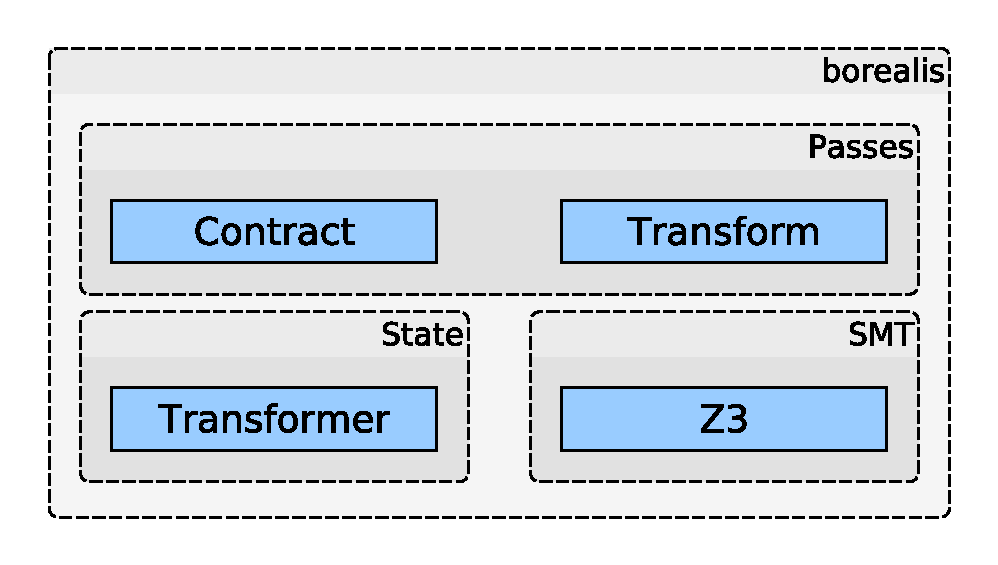
\includegraphics[width=0.75\linewidth]{borealisStructure}}
\caption{Структура модулей разрабатываемого прототипа}
\label{image:borealisStructure}
\end{figure}

Данный модуль основывается на предложенной ранее технологии автоматического извлечения контрактов. Он реализует следующие функции: анализ исходного кода и извлечение предварительного множества предикатов, работа с БД для записи/чтения результатов анализа, формирование контрактов для функции и добавление обнаруженных контрактов в систему для выполнения статического анализа.

Структура модулей библиотеки для работы с БД приведена ниже (см. рисунок \ref{image:leveldbStructure}). В данном проекте реализуются два подпроекта: сервер для непосредственной работы с БД и клиент для подключения к этому серверу.
\begin{figure}[h!]
\center{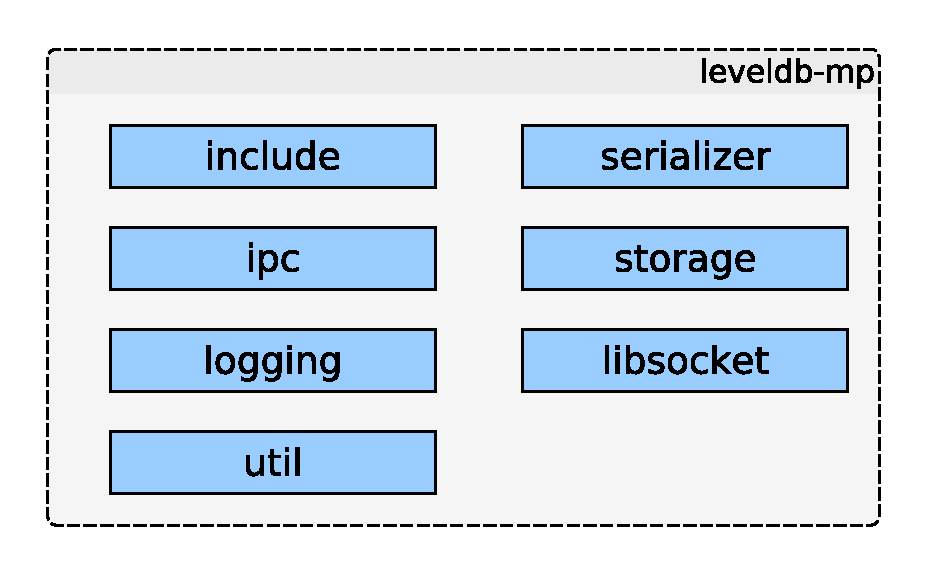
\includegraphics[width=0.75\linewidth]{leveldbStructure}}
\caption{Структура модулей библиотеки для работы с БД}
\label{image:leveldbStructure}
\end{figure}

%%%%%%%%%%%%%%%%%%%%%%%%%%%%%%%%%%%%%%%%%%%%%%%%%%%%%%%%%%%%%%%%%%%%%%%%%%%%%%%%
\section{Разработка библиотеки для взаимодействия с БД}
%%%%%%%%%%%%%%%%%%%%%%%%%%%%%%%%%%%%%%%%%%%%%%%%%%%%%%%%%%%%%%%%%%%%%%%%%%%%%%%%
LevelDB~\cite{leveldb} --- встраиваемая база данных, организованная как хранилище пар ключ-значение. Данное хранилище имеет ряд положительных качеств:
\begin{itemize}
\item БД является встраиваемой;
\item БД достаточно проста. Работа с ней происходит с помощью простых запросов put/get;
\item БД обладает высокой производительностью по сравнению с аналогами\footnote{http://leveldb.googlecode.com/svn/trunk/doc/benchmark.html};
\end{itemize}

LevelDB имеет один недостаток: она не поддерживает одновременное подключение нескольких процессов. Система Borealis может запускаться параллельно на нескольких проектах (или на нескольких модулях одного проекта), в таких случаях использование LevelDB может оказаться проблемой. Однако, подобная проблема присуща всем встраиваемым хранилищам.

Для решения проблемы одновременного подключения нескольких процессов было решено реализовать оболочку для хранилища, которая будет принимать запросы от нескольких клиентов и осуществлять непосредственное взаимодействие с хранилищем. Данная оболочка состоит из серверной и клиентской части. Серверная часть реализована в виде UNIX-демона. Клиентская часть компилируется в виде статической библиотеки. Рассмотрим компоненты данного модуля более подробно.

%%%%%%%%%%%%%%%%%%%%%%%%%%%%%%%%%%%%%%%%%%%%%%%%%%%%%%%%%%%%%%%%%%%%%%%%%%%%%%%%
\subsection{Компонент \texttt{storage}}
%%%%%%%%%%%%%%%%%%%%%%%%%%%%%%%%%%%%%%%%%%%%%%%%%%%%%%%%%%%%%%%%%%%%%%%%%%%%%%%%
В компоненте \texttt{storage} содержится класс \texttt{Database}, который выполняет непосредственное взаимодействие с БД. Для создания объекта класса \texttt{Database} требуется указать ему путь к БД. В качестве ключей используются строковый тип \texttt{std::string}, в качестве данных принимается объект типа \texttt{leveldb::Slice}, который содержит в себе массив байт и размер массива. Класс реализует следующие методы:
\begin{itemize}
\item \texttt{bool put(const Key\& key, Value value)} --- метод выполняет запись объекта в БД по полученному ключу. Возвращает \texttt{false}, в случае возникновения ошибки при записи.
\item \texttt{Value get(const Key\& key)} --- метод выполняет чтение данных из БД по ключу. Если объект в БД не найден, то метод вернет объект, размер которого равен 0.
\item \texttt{Iterator get(const Key\& from, const Key\& to)} --- метод выполняет чтение данных в интервале ключей. Возвращает объект типа \texttt{Database::Iterator}, который является оберткой для стандартного итератора библиотеки LevelDB.
\end{itemize}

Класс \texttt{Database::Iterator} реализует три метода: проверку на валидность \texttt{valid()}, переход к следующему объекту \texttt{next()} и получение объекта \texttt{value()}. Подобный интерфейс был выбран по образу стандартного итератора \texttt{leveldb::Iterator} из библиотеки LevelDB. Класс \texttt{Database::Iterator} является оберткой над \texttt{leveldb::Iterator} и добавляет к нему возможность итерирования по данным, ключ которых начинается с определенного значения.

%%%%%%%%%%%%%%%%%%%%%%%%%%%%%%%%%%%%%%%%%%%%%%%%%%%%%%%%%%%%%%%%%%%%%%%%%%%%%%%%
\subsection{Компонент \texttt{libsocket}}
%%%%%%%%%%%%%%%%%%%%%%%%%%%%%%%%%%%%%%%%%%%%%%%%%%%%%%%%%%%%%%%%%%%%%%%%%%%%%%%%
Для межпроцессного обмена используются UNIX-сокеты. Для работы с сокетами была использована библиотека libsocket~\cite{libsocket}, так как она предоставляет удобные инструменты для обмена данными и поддерживает UNIX-сокеты.

%%%%%%%%%%%%%%%%%%%%%%%%%%%%%%%%%%%%%%%%%%%%%%%%%%%%%%%%%%%%%%%%%%%%%%%%%%%%%%%%
\subsection{Компонент \texttt{ipc}}
%%%%%%%%%%%%%%%%%%%%%%%%%%%%%%%%%%%%%%%%%%%%%%%%%%%%%%%%%%%%%%%%%%%%%%%%%%%%%%%%
В данном компоненте содержатся классы, которые выполняют обмен по сети. Для обмена был разработан строковый сетевой протокол. Протокол содержит 6 команд: 
\begin{itemize}
\item \texttt{put} --- запись в БД;
\item \texttt{gto} --- чтение из БД по ключу;
\item \texttt{gta} --- получение из БД данных ключ которых начинается с указанного значения;
\item \texttt{end} --- завершение обмена;
\item \texttt{ok_} --- успешное выполнение команды;
\item \texttt{nok} --- ошибка.
\end{itemize}
Команда \texttt{put} использует два дополнительных аргумента: ключ и данные. Команды \texttt{gto} и \texttt{gta} требуют указания ключа. Каждая команда протокола занимает 3 байта. При отправке ключа и данных предварительно необходимо передать их размер, который передается в виде 8-разрядного шестнадцатеричного числа, преобразованного в строку. Схема пакета протокола приведена на рисунке \ref{image:packageStructure}
\begin{figure}[h!]
\center{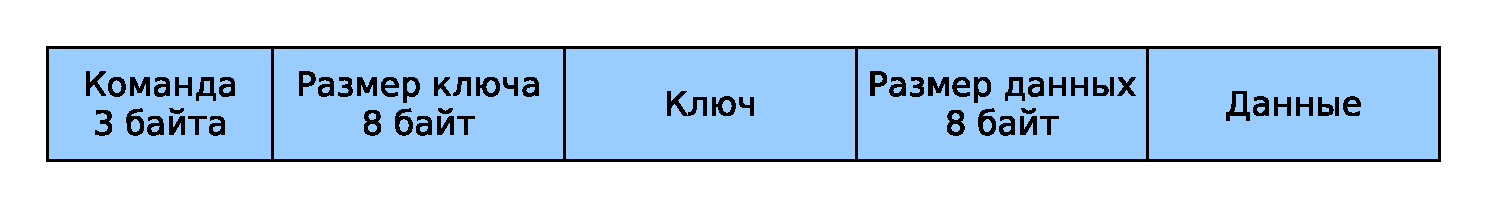
\includegraphics[width=\linewidth]{packageStructure}}
\caption{Схема пакета протокола}
\label{image:packageStructure}
\end{figure}

В данном компоненте реализовано два класса: \texttt{Server} и \texttt{Client}. \texttt{Server} реализует два метода: \texttt{work} --- основной цикл работы сервера и \texttt{destroy} --- уничтожение сокета. В основном цикле работы происходит обмен с клиентами. Синхронизация между клиентами выполняется на уровне подключения: сервер одновременно может выполнять обмен только с одним клиентом. Сервер запускается в виде UNIX-демона.

Класс \texttt{Client} содержит следующие методы: 
\begin{itemize}
\item \texttt{void connect(const std::string\& server)} --- подключение к серверу;
\item \texttt{bool put(const std::string\& key, char* data, size_t size)} --- передача данных серверу;
\item \texttt{std::pair<char*, size_t> get(const std::string\& key)} --- получение данных от сервера по ключу;
\item \texttt{DataArray getAll(const std::string\& key)} --- получение массива данных, ключи которых начинаются с переданного значения. \texttt{DataArray} определен как \texttt{std::vector< std::pair<char*, size_t> >};
\item \texttt{void close()} --- завершение соединения.
\end{itemize}

%%%%%%%%%%%%%%%%%%%%%%%%%%%%%%%%%%%%%%%%%%%%%%%%%%%%%%%%%%%%%%%%%%%%%%%%%%%%%%%%
\subsection{Компонент \texttt{include}}
%%%%%%%%%%%%%%%%%%%%%%%%%%%%%%%%%%%%%%%%%%%%%%%%%%%%%%%%%%%%%%%%%%%%%%%%%%%%%%%%
Данный компонент содержит заголовочные файлы для подключения библиотеки. В нем содержится файл DB.hpp, в котором реализован класс \texttt{DB}. Класс \texttt{DB} реализован в соответствии с паттерном Singleton~\cite{patterns} и содержит методы для работы с сервером:
\begin{itemize}
\item \texttt{static DB::Ptr getInstance()} --- получить экземпляр класса \texttt{DB};
\item \texttt{static bool isDaemonStarted()} --- метод, который проверяет запущен ли демон в системе;
\item \texttt{void setSocket(const std::string\& socket_name)} --- метод для задания сокета, к которому будут подключаться клиенты;
\item \texttt{void lock()} --- метод позволяет заблокировать сервер, чтобы ограничить подключение к нему других клиентов;
\item \texttt{void unlock()} --- разблокировать сервер;
\item \texttt{bool write(const std::string\& key, const T\& obj)} --- запись объекта в БД;
\item \texttt{ResT read(const std::string\& key, Context\& ctx)} --- чтение одиночного объекта из БД по ключу;
\item \texttt{std::vector<ResT> readAll(const std::string\& key, Context\& ctx)} --- чтение массива объектов из БД, ключ которых начинается с указанной последовательности.
\end{itemize}
Клиентская часть реализована в методах класса. Методы используют объект типа \texttt{ipc::Client} для подключения к серверу. Для взаимодействия с сервером пользователю необходимо лишь получить объект класса \texttt{DB}.


%%%%%%%%%%%%%%%%%%%%%%%%%%%%%%%%%%%%%%%%%%%%%%%%%%%%%%%%%%%%%%%%%%%%%%%%%%%%%%%%
\subsection{Вспомогательные компоненты}
%%%%%%%%%%%%%%%%%%%%%%%%%%%%%%%%%%%%%%%%%%%%%%%%%%%%%%%%%%%%%%%%%%%%%%%%%%%%%%%%
Проект также содержит несколько компонентов, которые реализуют дополнительные функции. Каталог \texttt{serializer} содержит шаблон структуры-сериализатора для любых объектов. Данный шаблон используется в клиентской части для сериализации/десериализации объектов при работе с БД. Для использования данного шаблона пользовательский класс должен реализовать следующий интерфейс:
\begin{itemize}
\item \texttt{static Buffer serialize(const T\& s)} --- метод сериализации, должен возвращать тип \texttt{serializer::Buffer};
\item \texttt{static ResultT deserialize(const SerializedT\& s, Context\& ctx)} --- метод десериализации. Принимает сериализованный объект и, при необходимости, контекст для десериализации;
\item \texttt{static ResultT notFound()} --- метод, который определяет возвращаемое значение в случае, когда объект не найден в БД.
\end{itemize}

Каталог \texttt{logging} содержит инструменты протоколирования работы программы. Каталог \texttt{util} содержит различные вспомогательные функции.

%%%%%%%%%%%%%%%%%%%%%%%%%%%%%%%%%%%%%%%%%%%%%%%%%%%%%%%%%%%%%%%%%%%%%%%%%%%%%%%%
\section{Разработка модуля для системы Borealis}
%%%%%%%%%%%%%%%%%%%%%%%%%%%%%%%%%%%%%%%%%%%%%%%%%%%%%%%%%%%%%%%%%%%%%%%%%%%%%%%%
В разработку модуля автоматического извлечения контрактов для системы Borealis входит написание новых классов для преобразования и анализа кода, а также расширение функциональности уже существующих классов.

В ходе работы были изменены несколько компонентов проекта (см. рисунок \ref{image:borealisStructure}). Компонент \texttt{Passes} содержит проходы LLVM, которые выполняют модификацию и преобразование исходного кода. Компонент \texttt{State} содержит описание и реализацию PS. Компонент \texttt{SMT} содержит инструменты для взаимодействия с SMT решателями.

%%%%%%%%%%%%%%%%%%%%%%%%%%%%%%%%%%%%%%%%%%%%%%%%%%%%%%%%%%%%%%%%%%%%%%%%%%%%%%%%
\subsection{Компонент \texttt{Passes}}
%%%%%%%%%%%%%%%%%%%%%%%%%%%%%%%%%%%%%%%%%%%%%%%%%%%%%%%%%%%%%%%%%%%%%%%%%%%%%%%%
В компонент \texttt{Passes} было внесено несколько изменений. Был добавлен проход \texttt{ContractExtractionPass}, который выполняет первоначальный анализ. В нем выполняется редукция предикатов равенства и извлекается изначальное множество предикатов для функции. \texttt{ContractExtractionPass} является \texttt{FunctionPass}, то есть выполняется на каждой функции модуля.

Были разработаны классы для работы с контрактами. Классы \texttt{Contract} и \texttt{ContractContainer} являются контейнерами и используются для хранения полученных контрактов, класс \texttt{FunctionIdentifier} используется для хранения информации о функции. 

Класс \texttt{Contract} представляет собой множество контрактов. Он содержит в себе вектор PS, которые были извлечены для функции. Класс \texttt{FunctionIdentifier} используется для представления функций. Он хранит имя,  тип возвращаемого значения (в виде строки), число вызовов функции и информацию о границах памяти функции (необходимо для последующей работы с SMT решателем). 

Класс \texttt{ContractContainer} используется для хранения результатов анализа. Он представляет из себя ассоциативный массив, ключами которого являются объекты типа \texttt{FunctionIdentifier}, а значениями --- объекты типа \texttt{Contract}. Для возможности хранения контрактов в БД для этих классов была реализована сериализация в формат Protocol Buffer~\cite{protobuf}. 

Кроме того, были разработаны два LLVM прохода: \texttt{ContractManager} и \texttt{ContractSummaryPass}. \texttt{ContractManager} является основным классом модуля. Он реализован в виде \texttt{ModulePass}. В нем хранятся все результаты анализа. Класс \texttt{ContractManager} реализует следующие методы:
\begin{itemize}
\item \texttt{void addContract(llvm::Function* F, FunctionManager\& FM, PredicateState::Ptr S, const std::unordered_map <int, Args>\& mapping)} --- добавить контракт для функции. Метод выполняет унификацию аргументов функции в PS, удаляет из него полные группы предикатов и сохраняет его;
\item \texttt{void saveState(FunctionIdentifier::Ptr func, PredicateState::Ptr state)} --- сохранить PS в \texttt{ContractContainer};
\item \texttt{Term::Ptr stateToTerm(PredicateState::Ptr state) const} --- преобразовать входной PS в терм. В общем случае такое преобразование невозможно, однако благодаря тому, что в виде контрактов извлекаются только предикаты равенства, любой PS в \texttt{ContractManager} можно преобразовать в терм. Эта операция используется для трансформации \texttt{PredicateStateChoice} в один предикат пути для возможности его сравнения с остальными результатами;
\item \texttt{void applyContracts() const} --- в методе выполняется слияние контрактов, печать полученных предусловий в файл и добавление их в систему для проверки;
\item \texttt{void printContractsDump()} --- печать полного множества предикатов в файл для отладки;
\item \texttt{void syncWithDB()} --- синхронизация множества предикатов с БД. Извлеченное множество предикатов объединяется с множеством из БД и снова сохраняется в БД. В процессе слияния двух множеств БД блокируется (чтобы избежать перезаписи данных).
\end{itemize}

Проход \texttt{ContractSummaryPass} --- это \texttt{ModulePass}, который используется для получения результатов анализа. Он вызывает метод \texttt{ContractManager::applyContracts()} после завершения всех остальных этапов анализа.

%%%%%%%%%%%%%%%%%%%%%%%%%%%%%%%%%%%%%%%%%%%%%%%%%%%%%%%%%%%%%%%%%%%%%%%%%%%%%%%%
\subsection{Компонент \texttt{State/Transformer}}
%%%%%%%%%%%%%%%%%%%%%%%%%%%%%%%%%%%%%%%%%%%%%%%%%%%%%%%%%%%%%%%%%%%%%%%%%%%%%%%%
Анализ и преобразование PS выполняется с помощью трансформеров (Transformer). Механизм трансформеров, используемый в системе Borealis, реализует паттерн CRTP (Curiously Recurring Template Pattern)~\cite{crtp} и паттерн Visitor~\cite{patterns}. Трансформеры являются удобным инструментом для анализа и трансформации PS. Они позволяют обходить как весь PS, так и его части (например, обходить только предикаты равенства).

Преобразования над PS, выполняемые в данной работе, также реализованы в виде трансформеров. Рассмотрим каждый трансформер более подробно.

\texttt{EqualityMapper} выполняет редукцию предикатов равенства (см. раздел \ref{subsection:reduction}). Трансформер выполняет обход всех предикатов равенства и предикатов пути (path predicates). В предикатах равенства запоминаются правые части выражений, в предикатах пути выполняется замена термов на их определения.

\texttt{ContractExtractorTransformer} выполняет анализ PS и извлечение первоначального множества контрактов. Трансформер обходит все предикаты в PS и оставляет в нем только предикаты, которые используют аргументы вызываемых функций. Таким образом, данный трансформер реализует алгоритм, представленный в разделе \ref{subsection:extraction}.

\texttt{ArgumentUnifier} производит унификацию аргументов функции. Он обходит все термы в PS и заменяет термы, которые соответствуют аргументам вызываемой функции, на \texttt{ArgumentTerm} с именами $arg\$i$, где $i$ --- номер аргумента (отсчет начинается с 0). Это необходимо для того, чтобы во всех найденных для функции предикатах передаваемые в нее переменные можно было идентифицировать как аргументы.

\texttt{ChoiceOptimizer} оптимизирует \texttt{PredicateStateChoice}: он удаляет в \texttt{PredicateStateChoice} пустые ветви, которые образуются в результате удаления предикатов в \texttt{ContractExtractorTransformer}.

\texttt{MergingTransformer} выполняет слияние предикатов. Он обходит все предикаты и выполняет поиск уникальных предикатов а также подсчет их количества. Далее, в методе \texttt{getMergedState} он реализует алгоритм слияния, представленный в разделе \ref{section:merging}. В методе \texttt{deleteOppositePredicates} выполняется удаление противоположных предикатов, в методе \texttt{mergePredicates} выполняется слияние оставшегося множества предикатов. Для сравнения предикатов данный трансформер использует SMT решатель Z3~\cite{z3solver}.

%%%%%%%%%%%%%%%%%%%%%%%%%%%%%%%%%%%%%%%%%%%%%%%%%%%%%%%%%%%%%%%%%%%%%%%%%%%%%%%%
\subsection{Компонент \texttt{SMT/Z3}}
%%%%%%%%%%%%%%%%%%%%%%%%%%%%%%%%%%%%%%%%%%%%%%%%%%%%%%%%%%%%%%%%%%%%%%%%%%%%%%%%
Для решения поставленных задач было решено использовать решатель Z3. В класс \texttt{Z3::Solver} было добавлено несколько новых методов:
\begin{itemize}
\item \texttt{smt::Result isFullGroup(PredicateState::Ptr query)} --- метод позволяет проверить образует ли PS полную группу событий. Для этого входной PS преобразуется в SMT формулу $f$. Затем формула $\bar{f}$ проверяется на выполнимость: если результат \texttt{unsat}, значит PS образует полную группу событий;
\item \texttt{z3::expr_vector getUnsatCore(std::vector<Predicate::Ptr>\& query, Predicate::Ptr pred)} --- метод используется для удаления противоположных предикатов и реализует алгоритм, представленный в разделе \ref{section:deleting};
\item \texttt{smt::Result isWeaker(Predicate::Ptr first, Predicate::Ptr second)} --- метод позволяет сравнить два предиката и определить, слабее ли первый предикат чем второй. Как указывалось ранее, для этого используется операция импликации (см. раздел \ref{section:merging}).
\end{itemize}

Данные методы используются другими классами проекта: \texttt{MergingTransformer} использует Z3 для слияния предикатов, \texttt{ContractManager} использует Z3 для удаления противоположных предикатов.

%%%%%%%%%%%%%%%%%%%%%%%%%%%%%%%%%%%%%%%%%%%%%%%%%%%%%%%%%%%%%%%%%%%%%%%%%%%%%%%%
\section{Резюме}
%%%%%%%%%%%%%%%%%%%%%%%%%%%%%%%%%%%%%%%%%%%%%%%%%%%%%%%%%%%%%%%%%%%%%%%%%%%%%%%%
В данном разделе рассмотрена реализация прототипа системы автоматического извлечения контрактов, основанного на предложенной технологии извлечения контрактов. Описаны основные составляющие прототипа: библиотека для взаимодействия с БД и модуль извлечения контрактов для системы Borealis. 